% Dissertation overview: conceptual research progression, not an implemented pipeline.
% Standalone source; all illustrations are editable TikZ paths.
% Rebuild from the repository root:
%   make figure-overview
\documentclass[tikz,border=3pt]{standalone}
\usepackage[T1]{fontenc}
\usepackage{newtxtext}
\usetikzlibrary{arrows.meta,calc}

% OpenTikZ light palette. One shared style for all four research modules.
\definecolor{otblue}{HTML}{0072B2}
\definecolor{otorange}{HTML}{E69F00}
\definecolor{otteal}{HTML}{009E73}
\definecolor{otpurple}{HTML}{CC79A7}
\definecolor{otgray}{HTML}{5A5A5A}

% Layout parameters (cm). Change these rather than individual card positions.
\def\CardWidth{3.65}
\def\CardGap{0.50}
\def\CardHeight{5.10}
\def\AxisY{5.87}
\def\AxisLabelY{6.50}
\def\PaperY{4.64}
\def\IconY{3.55}
\def\ThemeY{2.40}
\def\DetailY{1.37}
\def\SideRuleY{0.78}
\def\SideY{0.38}
\def\TextWidth{3.05cm}
\def\IconScale{0.91}

% Text parameters. Additional works are names only; MWM has no side work.
\def\SignalsLabel{Signals}
\def\SemanticsLabel{Semantics}
\def\ActionsLabel{Actions}
\def\HybridTitle{HyBRiD}
\def\MindTitle{MindLLM}
\def\MWMTitle{MWM}
\def\DystaTitle{DySta}
\def\HybridTheme{Modeling\\brain signals}
\def\MindTheme{From signals\\to semantics}
\def\MWMTheme{From semantics\\to action}
\def\DystaTheme{Acting in the\\physical world}
\def\HybridDetail{High-order brain\\relationships}
\def\MindDetail{Brain activity to\\semantic content}
\def\MWMDetail{Visual consequences\\as supervision}
\def\DystaDetail{Temporal memory\\and efficient action}
\def\HybridSide{SWA}
\def\MindSide{PRISM\enspace\textperiodcentered\enspace D-Edit}
\def\DystaSide{PHIL}

\tikzset{
  % Glyphs occupy a dedicated band, separate from every text label.
  pics/brain/.style={code={
    \path[draw=otblue!65!otgray,fill=otblue!5,line width=0.75pt]
      (-0.69,-0.31)
      .. controls (-1.03,-0.27) and (-1.08,0.05) .. (-0.89,0.22)
      .. controls (-1.02,0.50) and (-0.74,0.72) .. (-0.50,0.66)
      .. controls (-0.36,0.87) and (0.03,0.85) .. (0.13,0.64)
      .. controls (0.43,0.77) and (0.70,0.53) .. (0.65,0.30)
      .. controls (0.95,0.12) and (0.77,-0.19) .. (0.54,-0.20)
      .. controls (0.38,-0.45) and (0.08,-0.39) .. (-0.07,-0.25)
      .. controls (-0.29,-0.46) and (-0.55,-0.47) .. cycle;
    \draw[draw=otblue!40!otgray,line width=0.5pt]
      (-0.49,0.64) .. controls (-0.59,0.40) and (-0.34,0.38) .. (-0.43,0.14)
      (-0.82,0.23) .. controls (-0.57,0.28) and (-0.64,-0.03) .. (-0.48,-0.13)
      (0.11,0.62) .. controls (-0.03,0.37) and (0.24,0.31) .. (0.10,0.15)
      (0.61,0.29) .. controls (0.40,0.36) and (0.41,0.06) .. (0.23,-0.01);
  }},
  pics/hyperbrain/.style={code={
    \pic at (0.10,-0.14) {brain};
    \path[draw=otblue!75!otgray,fill=otblue!12,line width=0.6pt,rounded corners=8pt]
      (-0.65,0.02) -- (-0.14,0.47) -- (0.47,0.13) -- (0.26,-0.37) -- cycle;
    \draw[draw=otblue!65!otgray,line width=0.65pt]
      (-0.58,0.03) -- (-0.14,0.40) -- (0.40,0.12) -- (0.21,-0.29) -- (-0.58,0.03)
      (-0.14,0.40) -- (0.21,-0.29) -- (-0.13,-0.02) -- (0.40,0.12);
    \foreach \x/\y in {-0.58/0.03,-0.14/0.40,0.40/0.12,0.21/-0.29,-0.13/-0.02}{
      \fill[otblue!75!otgray] (\x,\y) circle[radius=2.1pt];
    }
  }},
  pics/semanticbridge/.style={code={
    \begin{scope}[shift={(-0.86,-0.10)},scale=0.63]
      \pic[scale=0.63] {brain};
      \foreach \x/\y in {-0.57/0.26,-0.22/0.47,0.16/0.12,-0.15/-0.10}{
        \fill[otblue!75] (\x,\y) circle[radius=2.5pt];
      }
    \end{scope}
    \draw[mini flow] (-0.23,0.03) -- (0.22,0.03);
    \path[draw=otblue!65!otgray,fill=otblue!5,line width=0.8pt,rounded corners=2pt]
      (0.36,-0.26) -- (0.36,0.41) -- (1.34,0.41) -- (1.34,-0.26)
      -- (0.76,-0.26) -- (0.52,-0.43) -- (0.54,-0.26) -- cycle;
    \foreach \y/\end in {0.24/1.15,0.06/1.15,-0.12/0.96}{
      \draw[draw=otblue!65!otgray,line width=0.9pt,line cap=round]
        (0.54,\y) -- (\end,\y);
    }
  }},
  pics/worlddynamics/.style={code={
    % EEG conditions prediction; observed visual consequences supervise learning.
    % Dashed feedback denotes training, not video-to-action inference.
    \draw[draw=otblue!70!otgray,line width=0.8pt,line join=round]
      (-0.46,0.65) -- (-0.31,0.65) -- (-0.23,0.80) -- (-0.12,0.45)
      -- (-0.01,0.72) -- (0.07,0.65) -- (0.33,0.65);
    \draw[mini flow] (-0.05,0.40) -- (-0.05,0.07);
    \foreach \x in {-1.34,0.38}{
      \path[draw=otblue!65!otgray,fill=otblue!5,line width=0.7pt,rounded corners=1.5pt]
        (\x,-0.48) rectangle +(0.96,0.70);
      \draw[draw=otgray!50,line width=0.55pt] (\x+0.10,-0.35) -- (\x+0.86,-0.35);
    }
    \path[draw=otblue!80!otgray,fill=otblue!25,line width=0.7pt]
      (-1.13,-0.35) rectangle + (0.24,0.24);
    \path[draw=otblue!80!otgray,fill=otblue!25,line width=0.7pt]
      (0.92,-0.35) rectangle + (0.24,0.24);
    \draw[mini flow] (-0.28,-0.12) -- (0.26,-0.12);
    \draw[mini flow,dashed] (0.86,0.29)
      .. controls (0.86,0.66) and (0.69,0.73) .. (0.39,0.73);
    \node[font=\fontsize{6}{7}\selectfont,text=otgray]
      at (1.30,0.72) {supervise};
  }},
  pics/memoryaction/.style={code={
    % Visual history and an articulated robot arm, not a brain-control loop.
    \foreach \x/\y in {-1.33/0.04,-1.22/-0.08,-1.11/-0.20}{
      \path[draw=otblue!55!otgray,fill=otblue!3,line width=0.65pt,rounded corners=1pt]
        (\x,\y) rectangle +(0.64,0.60);
    }
    \draw[draw=otblue!70!otgray,line width=0.65pt]
      (-1.00,-0.09) -- (-0.86,0.12) -- (-0.73,-0.02) -- (-0.59,0.18);
    \draw[mini flow] (-0.32,0.06) -- (0.12,0.06);
    \path[draw=otblue!65!otgray,fill=otblue!12,line width=0.8pt,rounded corners=1.5pt]
      (0.31,-0.46) rectangle +(0.50,0.15);
    \draw[draw=otblue!65!otgray,line width=4pt,line cap=round,line join=round]
      (0.56,-0.31) -- (0.39,0.22) -- (0.94,0.53) -- (1.28,0.19);
    \draw[draw=otblue!12,line width=2.4pt,line cap=round,line join=round]
      (0.56,-0.31) -- (0.39,0.22) -- (0.94,0.53) -- (1.28,0.19);
    \foreach \x/\y in {0.56/-0.31,0.39/0.22,0.94/0.53}{
      \filldraw[draw=otblue!65!otgray,fill=otblue!4,line width=0.7pt]
        (\x,\y) circle[radius=2.1pt];
    }
    \draw[draw=otblue!65!otgray,line width=0.85pt]
      (1.16,0.12) -- (1.16,-0.01) -- (1.23,-0.08)
      (1.40,0.12) -- (1.40,-0.01) -- (1.33,-0.08)
      (1.16,0.12) -- (1.40,0.12);
    \path[draw=otblue!65!otgray,fill=otblue!20,line width=0.65pt]
      (1.15,-0.43) rectangle +(0.27,0.23);
  }}
}

\begin{document}
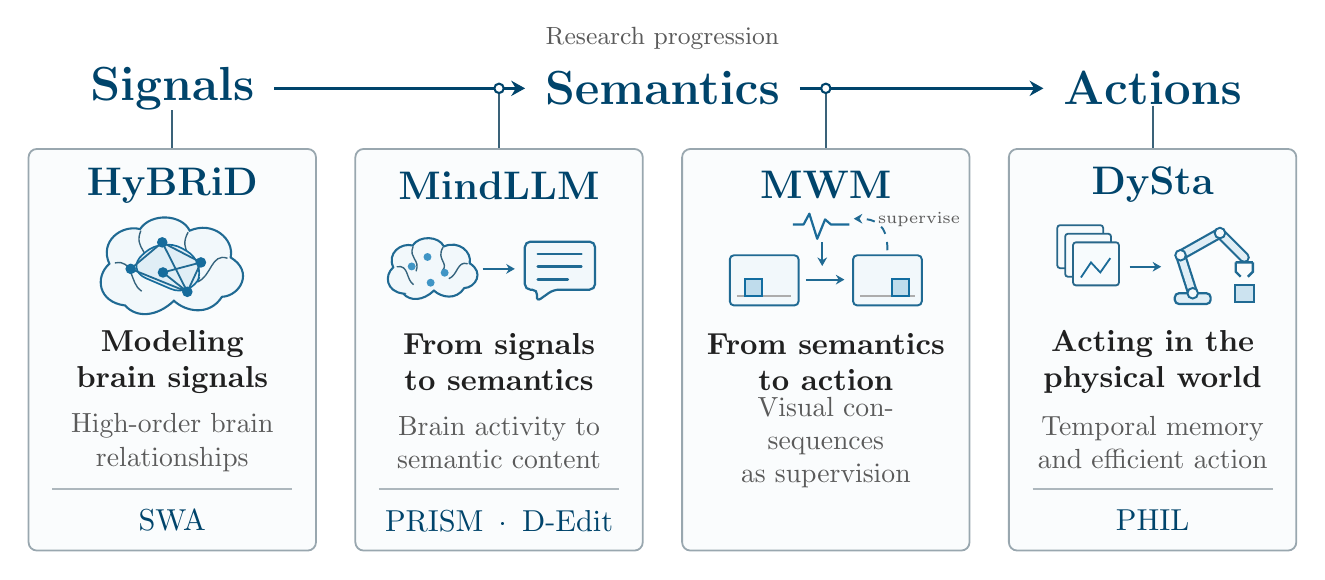
\begin{tikzpicture}[x=1cm,y=1cm,
  every node/.style={inner sep=0pt,align=center,text=otgray!35!black},
  concept/.style={font=\fontsize{17}{19}\selectfont\bfseries,text=otblue!60!black},
  paper/.style={font=\fontsize{14}{16}\selectfont\bfseries,text=otblue!60!black},
  theme/.style={font=\fontsize{11}{13}\selectfont\bfseries,text width=\TextWidth},
  detail/.style={font=\fontsize{10}{12}\selectfont,text=otgray,text width=\TextWidth},
  side/.style={font=\fontsize{10.5}{12}\selectfont,text=otblue!60!black},
  progression/.style={-{Stealth[length=5pt,width=5.5pt]},draw=otblue!60!black,line width=1.0pt},
  mini flow/.style={-{Stealth[length=3.1pt,width=3.5pt]},draw=otblue!65!otgray,line width=0.7pt},
  stem/.style={draw=otblue!35!otgray,line width=0.7pt},
  module/.style={draw=otblue!23!otgray!55,fill=otblue!2,line width=0.65pt,rounded corners=3pt}
]
\pgfmathsetmacro{\CardStep}{\CardWidth+\CardGap}
\pgfmathsetmacro{\HybridX}{0.5*\CardWidth}
\pgfmathsetmacro{\MindX}{\HybridX+\CardStep}
\pgfmathsetmacro{\MWMX}{\HybridX+2*\CardStep}
\pgfmathsetmacro{\DystaX}{\HybridX+3*\CardStep}
\pgfmathsetmacro{\CenterX}{0.5*(\HybridX+\DystaX)}

% Research axis: endpoint works attach to the endpoint concepts; bridge works
% attach to the line segments. No arrows run between the four model modules.
\node[font=\fontsize{9}{11}\selectfont,text=otgray] (research-progression)
  at (\CenterX,\AxisLabelY) {Research progression};
\node[concept] (signals) at (\HybridX,\AxisY) {\SignalsLabel};
\node[concept] (semantics) at (\CenterX,\AxisY) {\SemanticsLabel};
\node[concept] (actions) at (\DystaX,\AxisY) {\ActionsLabel};
\draw[progression,shorten <=7pt,shorten >=7pt] (signals.east) -- (semantics.west);
\draw[progression,shorten <=7pt,shorten >=7pt] (semantics.east) -- (actions.west);
\draw[stem] (signals.south) -- (\HybridX,\CardHeight);
\draw[stem] (actions.south) -- (\DystaX,\CardHeight);
\foreach \x/\name in {\MindX/mindllm-bridge,\MWMX/mwm-bridge}{
  \coordinate (\name) at (\x,\AxisY);
  \draw[stem] (\name) -- (\x,\CardHeight);
  \filldraw[fill=otblue!0,draw=otblue!60!black,line width=0.75pt]
    (\name) circle[radius=1.7pt];
}

% Equal-width modules with independent title, glyph, theme, detail, and footer.
\foreach \x/\name/\title/\theme/\detail/\glyph in {
  \HybridX/hybrid/\HybridTitle/\HybridTheme/\HybridDetail/hyperbrain,
  \MindX/mindllm/\MindTitle/\MindTheme/\MindDetail/semanticbridge,
  \MWMX/mwm/\MWMTitle/\MWMTheme/\MWMDetail/worlddynamics,
  \DystaX/dysta/\DystaTitle/\DystaTheme/\DystaDetail/memoryaction}{
  \node[module,minimum width=\CardWidth cm,minimum height=\CardHeight cm]
    (\name-card) at (\x,{0.5*\CardHeight}) {};
  \node[paper] (\name-title) at (\x,\PaperY) {\title};
  \pic[scale=\IconScale] (\name-icon) at (\x,\IconY) {\glyph};
  \node[theme] (\name-theme) at (\x,\ThemeY) {\theme};
  \node[detail] (\name-detail) at (\x,\DetailY) {\detail};
}
\foreach \x/\name/\label in {
  \HybridX/hybrid/\HybridSide,\MindX/mindllm/\MindSide,\DystaX/dysta/\DystaSide}{
  \draw[draw=otblue!20!otgray!45,line width=0.5pt]
    (\x-0.5*\CardWidth+0.30,\SideRuleY) -- (\x+0.5*\CardWidth-0.30,\SideRuleY);
  \node[side] (\name-additional) at (\x,\SideY) {\label};
}
\end{tikzpicture}
\end{document}
